\chapter{संकुलों के इलेक्ट्रॉनिक स्पेक्ट्रम और चुंबकत्व}\label{ch:b3:complex-spectra-magnetism}

माणिक लाल है और पन्ना हरा, फिर भी दोनों अपना रंग एक ही आयन,
\ce{Cr^{3+}}, के कारण पाते हैं, जो दो भिन्न ऑक्साइडों में कुछ ऐलुमिनियम आयनों का स्थान लेता है: माणिक के लिए
कुरुंद, $\ce{Al2O3}$, और पन्ने के लिए बेरिलियम ऐलुमिनियम सिलिकेट बेरिल।
दोनों में क्रोमियम ऑक्सीजन परमाणुओं के एक अष्टफलक में बैठा है; बेरिल में
अष्टफलक थोड़ा बड़ा है और लिगैंड क्षेत्र थोड़ा दुर्बल, और आयन के
अवशोषण बैंड लगभग एक हज़ार तरंग-संख्याएँ लाल की ओर खिसक जाते हैं।
पारगत रंग को लाल से हरे में बदलने के लिए इतना पर्याप्त है। यह अध्याय
ऐसे स्पेक्ट्रमों की मात्रात्मक व्याख्या करता है: किसी मुक्त आयन के पद लिगैंड क्षेत्र में कैसे
विपाटित होते हैं, \omterm{def:b3:complex-spectra-magnetism:tanabe-sugano}{तानाबे--सुगानो आरेख} दो बैंड स्थितियों को
लिगैंड-क्षेत्र विपाटन और इलेक्ट्रॉन प्रतिकर्षण में कैसे बदलते हैं, कुछ बैंड तीव्र
और अन्य क्षीण क्यों होते हैं, कुछ संकुल विकृत क्यों होते हैं, और चुंबकत्व
अयुग्मित इलेक्ट्रॉनों की गिनती कैसे करता है।

\begin{recall}
द्वितीय वर्ष के खंड ने संक्रमण तत्वों और उनके $d^n$ विन्यासों,
क्रिस्टल-क्षेत्र विपाटन $\Delta_{\mathrm o}$, उच्च- और निम्न-चक्रण संकुलों, युग्मन ऊर्जा,
क्रिस्टल-क्षेत्र स्थायीकरण ऊर्जा, $d$--$d$ संक्रमणों, स्पेक्ट्रमरासायनिक
श्रेणी, लिगैंड क्षेत्र सिद्धांत, तथा अनुचुंबकीय और प्रतिचुंबकीय पदार्थों का विवेचन किया।
\Cref{ch:b3:many-electron-atoms} ने \omterm{def:b3:many-electron-atoms:term}{पद प्रतीक} और हुंड के नियम व्युत्पन्न किए,
\cref{ch:b3:group-theory-applied} ने निरूपणों का लघुकरण और \omterm{def:b3:group-theory-applied:direct-product}{प्रत्यक्ष गुणनफल} दिए,
\cref{ch:b3:electronic-spectroscopy} ने चक्रण और लापोर्ट वरण नियम बताए
और \omterm{def:b3:electronic-spectroscopy:charge-transfer}{आवेश-स्थानांतरण संक्रमणों} का वर्णन किया, तथा
\cref{ch:b3:partition-functions} ने \omterm{def:b3:partition-functions:boltzmann}{बोल्ट्समान वितरण} दिया।
\end{recall}

\begin{omfigure}
\begin{minipage}[b]{0.3\linewidth}\centering
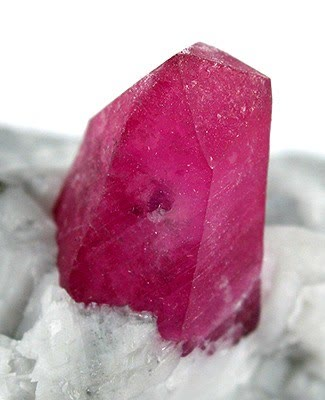
\includegraphics[height=4.2cm]{images/book4/ruby-crystal.jpg}\par
{\small माणिक}
\end{minipage}\hspace{1.5em}
\begin{minipage}[b]{0.3\linewidth}\centering
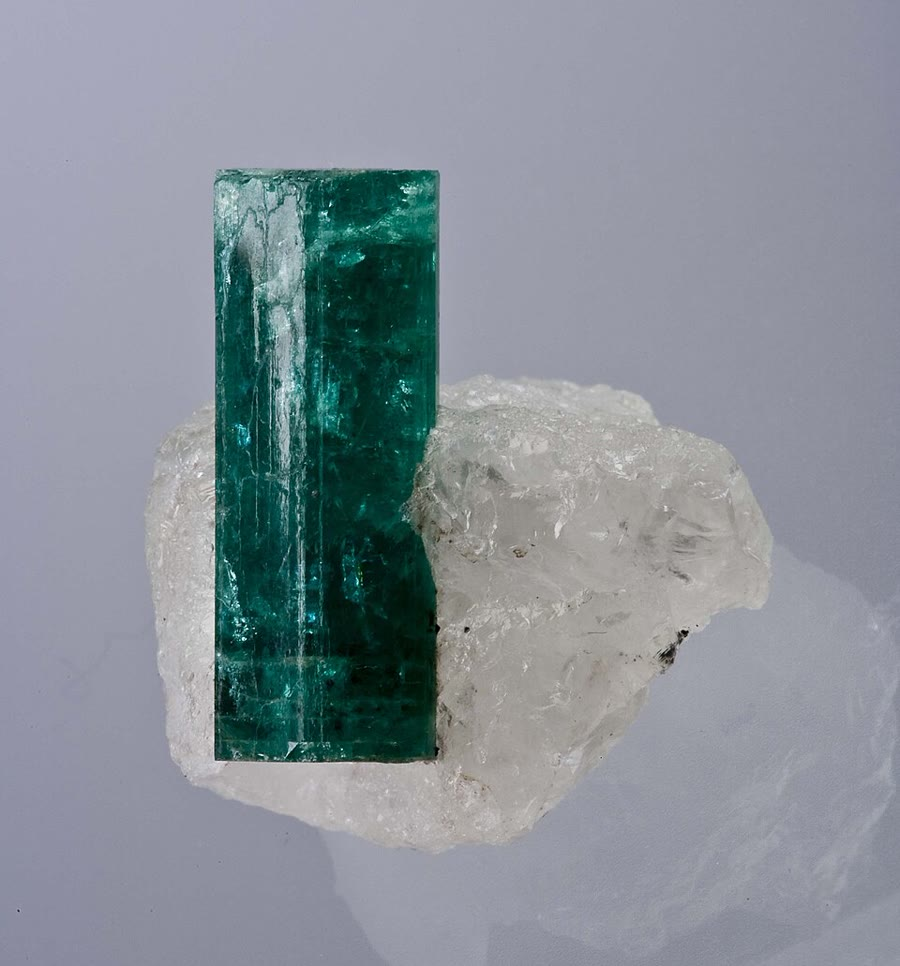
\includegraphics[height=4.2cm]{images/book4/emerald-crystal.jpg}\par
{\small पन्ना}
\end{minipage}

{\small संगमरमर में एक माणिक क्रिस्टल और क्वार्ट्ज़ पर एक पन्ना क्रिस्टल। दोनों में
रंग अष्टफलकीय स्थल में स्थित कुछ प्रतिशत \ce{Cr^{3+}} से आता है।}
\end{omfigure}

\section{मुक्त-आयन पदों से लिगैंड-क्षेत्र पदों तक}

मुक्त आयन में इलेक्ट्रॉन प्रतिकर्षण किसी $d^n$ विन्यास को पदों में विपाटित करता है
($^4$F, $^4$P, $^2$G\dots, $d^3$ के लिए, \cref{ch:b3:many-electron-atoms})। संकुल में प्रत्येक पद
लिगैंडों द्वारा और विपाटित होता है, और स्तरों को संकुल के \omterm{def:b3:point-groups:point-group}{बिंदु समूह} के \omterm{def:b3:point-groups:irrep}{अलघुकरणीय
निरूपणों} से नामांकित किया जाता है।

\begin{definition}[लिगैंड-क्षेत्र पद]\label{def:b3:complex-spectra-magnetism:ligand-field-term}
किसी संकुल का \emph{लिगैंड-क्षेत्र पद}\index{लिगैंड-क्षेत्र पद} अपभ्रष्ट
बहु-इलेक्ट्रॉन अवस्थाओं का वह समुच्चय है जिसे उसकी \omterm{def:b3:many-electron-atoms:term}{चक्रण बहुकता} और \omterm{def:b3:point-groups:point-group}{बिंदु समूह} के उस
\omterm{def:b3:point-groups:irrep}{अलघुकरणीय निरूपण} से नामांकित किया जाता है जिससे उसका कक्षकीय भाग
संबंधित है, जैसे अष्टफलकीय संकुल में $^4$A$_{2g}$ या $^4$T$_{1g}$।
\end{definition}

\begin{proposition}[घूर्णन समूह के अभिलक्षण]\label{prop:b3:complex-spectra-magnetism:rotation-characters}
किसी पद की $2L+1$ अवस्थाएँ, जिसका कक्षीय कोणीय संवेग $L$ है, घूर्णनों का एक निरूपण
बनाती हैं, जिसका कोण $\alpha$ से घूर्णन के लिए \omterm{def:b3:point-groups:representation}{अभिलक्षण} है
\[
  \chi_L(\alpha) = \frac{\sin\bigl((L + \tfrac12)\alpha\bigr)}{\sin(\alpha/2)}, \qquad \chi_L(0) = 2L + 1 .
\]
\end{proposition}

\admitted

\begin{theorem}[अष्टफलकीय क्षेत्र में मुक्त-आयन पदों का विपाटन]\label{thm:b3:complex-spectra-magnetism:term-splitting}
अष्टफलकीय क्षेत्र में किसी $d^n$ आयन के पद इस प्रकार विपाटित होते हैं
\begin{center}
\begin{tabular}{ll}
\hline
मुक्त-आयन पद & अष्टफलकीय पद (वही \omterm{def:b3:many-electron-atoms:term}{चक्रण बहुकता}) \\ \hline
S & A$_{1g}$ \\
P & T$_{1g}$ \\
D & E$_g$ + T$_{2g}$ \\
F & A$_{2g}$ + T$_{1g}$ + T$_{2g}$ \\
G & A$_{1g}$ + E$_g$ + T$_{1g}$ + T$_{2g}$ \\ \hline
\end{tabular}
\end{center}
\end{theorem}

\begin{proof}
अष्टफलकीय समूह घूर्णन समूह $O$ गुणा प्रतिलोमन है; $d$ फलन
सम हैं, अतः किसी $d^n$ विन्यास का हर पद सम ($g$) है, और
$O$ में लघुकरण पर्याप्त है, जिसके वर्ग $E$, $8C_3$, $3C_2$ ($=C_4^2$), $6C_4$ और $6C_2'$ हैं।
प्रस्ताव से, $L = 3$ के लिए: $\chi = 7$, $\sin(420^\circ)/\sin60^\circ = 1$, $\sin(630^\circ)/\sin90^\circ = -1$, $\sin(315^\circ)/\sin45^\circ = -1$
और $-1$। $O$ की \omterm{def:b3:point-groups:irrep}{अभिलक्षण सारणी} (पंक्तियाँ $A_1$: 1, 1, 1, 1, 1; $A_2$: 1, 1, 1, $-1$, $-1$; $E$: 2,
$-1$, 2, 0, 0; $T_1$: 3, 0, $-1$, 1, $-1$; $T_2$: 3, 0, $-1$, $-1$, 1) और
\cref{ch:b3:group-theory-applied} का \omterm{thm:b3:group-theory-applied:reduction}{लघुकरण सूत्र} $n(A_2) = (7 + 8 - 3 + 6 + 6)/24 = 1$, $n(T_1) = (21 + 3 - 6 +
6)/24 = 1$, $n(T_2) = (21 + 3 + 6 - 6)/24 = 1$ देते हैं, और $A_1$ तथा $E$ के लिए शून्य। अन्य पंक्तियाँ
इसी प्रकार प्राप्त होती हैं ($L = 0$: $(1, 1, 1, 1, 1)$; $L = 1$: $(3, 0, -1, 1, -1)$; $L = 2$: $(5, -1, 1,
-1, 1)$; $L = 4$: $(9, 0, 1, 1, 1)$)।
\end{proof}

\begin{method}[किसी मुक्त-आयन पद का विपाटन]\label{met:b3:complex-spectra-magnetism:split-term}
\begin{enumerate}
  \item मुक्त आयन का मूल पद (हुंड के नियम) और उसी बहुकता के उत्तेजित
        पद ज्ञात कीजिए।
  \item सारणी में उनके अष्टफलकीय घटक पढ़िए; \omterm{def:b3:many-electron-atoms:term}{चक्रण बहुकता}
        अपरिवर्तित रहती है।
  \item उन्हें क्रम में रखिए: $d^2$, $d^7$ (उच्च चक्रण) के मूल F पद के लिए सबसे निम्न T$_{1g}$ है;
        $d^3$, $d^8$ के लिए A$_{2g}$ (अगला प्रस्ताव)।
\end{enumerate}
\end{method}

\begin{proposition}[छिद्र और चतुष्फलकीय व्युत्क्रमण]\label{prop:b3:complex-spectra-magnetism:hole}
अष्टफलकीय क्षेत्र में $d^{10-n}$ के पद, उलटे ऊर्जा
क्रम में, $d^n$ के पद ही हैं; चतुष्फलकीय क्षेत्र में $d^n$ के पद अष्टफलकीय
क्षेत्र में $d^{10-n}$ के पद हैं ($g$ पादांक हटाकर)।
\end{proposition}

\begin{proof}
एक $d^{10-n}$ विन्यास पूर्ण कोश में $n$ धनात्मक छिद्रों के तुल्य है:
छिद्र लिगैंड-क्षेत्र विभव को विपरीत चिह्न के साथ अनुभव करते हैं, अतः प्रत्येक
एक-इलेक्ट्रॉन विपाटन, और फलतः प्रत्येक पद विपाटन, उलट जाता है (छिद्रों के बीच
इलेक्ट्रॉन प्रतिकर्षण इलेक्ट्रॉनों के बीच जैसा ही है)। चतुष्फलकीय
क्षेत्र का चिह्न अष्टफलकीय क्षेत्र के विपरीत होता है ($e$ कक्षक
नीचे रहते हैं) और उसमें सममिति केंद्र नहीं होता: $d^n$, $T_d$ में, उलटे
क्षेत्र वाले $d^n$ की तरह व्यवहार करता है, अर्थात् $d^{10-n}$ की तरह, $O_h$ में।
\end{proof}

\begin{definition}[सहसंबंध आरेख]\label{def:b3:complex-spectra-magnetism:correlation}
\emph{सहसंबंध आरेख}\index{सहसंबंध आरेख} किसी निकाय की दो सीमांत स्थितियों की
अवस्थाओं को जोड़ता है, यहाँ दुर्बल क्षेत्र द्वारा विपाटित मुक्त-आयन पद
और प्रबल क्षेत्र के विन्यास $t_{2g}^ae_g^b$, और यह समान सममिति की
अवस्थाओं को इस प्रकार जोड़ता है कि उनमें से कोई दो एक-दूसरे को न काटें।
\end{definition}

\begin{omfigure}
\begin{tikzpicture}[font=\small]
  % free ion
  \pic (F) at (0,0) {omlevel={}{1.1}};
  \pic (P) at (0,3.0) {omlevel={}{1.1}};
  \node[anchor=east] at (F-l) {$^3$F};
  \node[anchor=east] at (P-l) {$^3$P};
  % weak field
  \pic (a) at (2.6,-0.8) {omlevel={}{1.0}};
  \pic (b) at (2.6,0.3) {omlevel={}{1.0}};
  \pic (c) at (2.6,1.4) {omlevel={}{1.0}};
  \pic (d) at (2.6,3.1) {omlevel={}{1.0}};
  \foreach \n/\t in {a/T$_{1g}$, b/T$_{2g}$, c/A$_{2g}$, d/T$_{1g}$(P)}{\node[omsymlabel, anchor=south] at (\n-c) {$^3$\t};}
  \draw[omcorr] (F-r) -- (a-l) (F-r) -- (b-l) (F-r) -- (c-l) (P-r) -- (d-l);
  % strong field configurations
  \pic (A) at (7.4,-1.6) {omlevel={}{1.0}};
  \pic (B) at (7.4,1.4) {omlevel={}{1.0}};
  \pic (C) at (7.4,1.9) {omlevel={}{1.0}};
  \pic (D) at (7.4,4.6) {omlevel={}{1.0}};
  \node[anchor=west] at (A-r) {$^3$T$_{1g}$ \quad $t_{2g}^2$};
  \node[anchor=west] at (B-r) {$^3$T$_{2g}$};
  \node[anchor=west] at (C-r) {$^3$T$_{1g}$ \quad $t_{2g}e_g$};
  \node[anchor=west] at (D-r) {$^3$A$_{2g}$ \quad $e_g^2$};
  \draw[omcorr] (a-r) -- (A-l) (b-r) -- (B-l) (c-r) -- (D-l) (d-r) -- (C-l);
  \node[anchor=north] at (0,-2.0) {मुक्त आयन};
  \node[anchor=north] at (2.6,-2.0) {दुर्बल क्षेत्र};
  \node[anchor=north] at (7.4,-2.0) {प्रबल क्षेत्र};
  \draw[->, black!50] (3.7,-2.3) -- (6.2,-2.3) node[midway, below, font=\scriptsize] {बढ़ता $\Delta_{\mathrm o}$};
\end{tikzpicture}

{\small अष्टफलकीय क्षेत्र में किसी $d^2$ आयन की \omterm{def:b3:many-electron-atoms:singlet-triplet}{त्रिक अवस्थाओं} का \omterm{def:b3:complex-spectra-magnetism:correlation}{सहसंबंध
आरेख}। प्रत्येक दुर्बल-क्षेत्र पद उसी सममिति के प्रबल-क्षेत्र विन्यास तक जाता है,
और दोनों $^3$T$_{1g}$ अवस्थाएँ एक-दूसरे को नहीं काटतीं: निचली $t_{2g}^2$ तक जाती है, ऊपरी
$t_{2g}e_g$ तक।}
\end{omfigure}

\section{तानाबे--सुगानो आरेख}

\begin{definition}[राका प्राचल]\label{def:b3:complex-spectra-magnetism:racah}
\emph{राका प्राचल}\index{राका प्राचल} $A$, $B$ और $C$, $d$ कोश के स्लेटर समाकलों के
वे संयोजन हैं जो किसी $d^n$ विन्यास की सभी इलेक्ट्रॉन-प्रतिकर्षण
ऊर्जाएँ व्यक्त करते हैं; एक ही विन्यास के पदों के बीच ऊर्जा अंतर
केवल $B$ और $C$ पर निर्भर करते हैं, और उसी
उच्चतम बहुकता के पदों के बीच के अंतर केवल $B$ पर ($d^2$, $d^3$, $d^7$, $d^8$ के लिए: $E(\mathrm P) - E(\mathrm F) = 15B$)।
\end{definition}

\begin{example}[मुक्त-आयन राका प्राचल]\label{ex:b3:complex-spectra-magnetism:free-B}
% ledger: lev:Cr3.4F5_2, lev:Cr3.4F7_2, lev:Cr3.4F9_2, lev:Cr3.4P1_2, lev:Cr3.4P3_2, lev:Cr3.4P5_2, lev:Ni2.3F3, lev:Ni2.3F2, lev:Ni2.3P2, lev:Ni2.3P1, lev:Ni2.3P0, lev:V2.4F5_2, lev:V2.4F7_2, lev:V2.4F9_2, lev:V2.4P1_2, lev:V2.4P3_2, lev:V2.4P5_2
मुक्त \ce{Cr^{3+}} आयन के स्तरों से गुरुत्व केंद्र (भार $2J + 1$) $^4$F के लिए
मूल स्तर से \qty{547}{cm^{-1}} ऊपर और $^4$P के लिए \qty{14305}{cm^{-1}} ऊपर आता है: $15B = \qty{13758}{cm^{-1}}$,
$B = \qty{917}{cm^{-1}}$। यही परिकलन \ce{V^{2+}} के लिए $B = 755$ और
\ce{Ni^{2+}} के लिए \qty{1056}{cm^{-1}} देता है।
\end{example}

\begin{definition}[तानाबे--सुगानो आरेख]\label{def:b3:complex-spectra-magnetism:tanabe-sugano}
\emph{तानाबे--सुगानो आरेख}\index{तानाबे--सुगानो आरेख} किसी $d^n$ आयन के सभी
\omterm{def:b3:complex-spectra-magnetism:ligand-field-term}{लिगैंड-क्षेत्र पदों} की ऊर्जाओं को, $B$ की इकाइयों में और
मूल पद से मापकर, $\Delta_{\mathrm o}/B$ के विरुद्ध, एक नियत अनुपात $C/B$ के लिए, आलेखित करता है।
\end{definition}

\begin{proposition}[$d^3$ आयन के तीन बैंड]\label{prop:b3:complex-spectra-magnetism:d3-bands}
अष्टफलकीय क्षेत्र में किसी $d^3$ आयन के लिए $^4$A$_{2g}$ से चक्रण-अनुमत संक्रमण यहाँ होते हैं:
\[
  \nu_1 = \Delta_{\mathrm o}\ (^4\mathrm T_{2g}), \qquad
  \nu_{2,3} = 7.5B + 1.5\Delta_{\mathrm o} \mp \tfrac12\sqrt{225B^2 - 18B\Delta_{\mathrm o} + \Delta_{\mathrm o}^2}\ (^4\mathrm T_{1g}(\mathrm F), {}^4\mathrm T_{1g}(\mathrm P)).
\]
\end{proposition}

\begin{proof}[आंशिक उपपत्ति]
प्रबल-क्षेत्र आधार में $^4$A$_{2g}$ और $^4$T$_{2g}$ एक-एक बार उत्पन्न होते हैं, $t_{2g}^3$ और $t_{2g}^2e_g$ से, और
उनके अंतर में कोई इलेक्ट्रॉन प्रतिकर्षण नहीं होता: ठीक $\nu_1 = \Delta_{\mathrm o}$। $^4$T$_{1g}$ दो बार
उत्पन्न होता है, $t_{2g}^2e_g$ और $t_{2g}e_g^2$ से; $^4$A$_{2g}$ के सापेक्ष $2\times2$ आव्यूह है
$\begin{pmatrix}\Delta_{\mathrm o} + 12B & 6B\\ 6B & 2\Delta_{\mathrm o} + 3B\end{pmatrix}$ (इलेक्ट्रॉन-प्रतिकर्षण अवयव स्वीकृत हैं)।
इसके \omterm{def:b3:quantum-model-systems:operator}{अभिलक्षणिक मान} $E^2 - (15B + 3\Delta_{\mathrm o})E + 2\Delta_{\mathrm o}^2 + 27B\Delta_{\mathrm o} = 0$ के मूल हैं, जो बताए गए
$\nu_2$ और $\nu_3$ हैं। $\Delta_{\mathrm o} = 0$ पर वे 0 और $15B$ हैं ($^4$F और $^4$P पद); चित्र का पूर्ण
विकर्णीकरण उन्हें पुनरुत्पन्न करता है।
\end{proof}

\begin{omfigure}
\begin{tikzpicture}
\begin{axis}[name=ta, omts, width=0.46\linewidth, height=7.0cm, xmin=1, xmax=40, ymin=0, ymax=70,
  xlabel={$\Delta_{\mathrm o}/B$}, ylabel={$E/B$}, title={\small $d^3$, $C/B = 4.5$},
  unbounded coords=jump, clip=true, clip mode=individual]
\foreach \c in {f0,f1,f2,f3,f4,f5,f6,f7,f8,f9,f10,f11,f12,f13,f14,f15}{
  \addplot[omtsforbidden, restrict x to domain=1:40] table[x=x, y=\c] {figdata/out/bachelor-3-tanabe-sugano-d3.dat};}
\foreach \c in {a0,a1,a2,a3}{
  \addplot[omDef, thick, restrict x to domain=1:40] table[x=x, y=\c] {figdata/out/bachelor-3-tanabe-sugano-d3.dat};}
\draw[omThm, dashed] (axis cs:29.0,0) -- (axis cs:29.0,70);
\draw[black!70, dashed] (axis cs:27.1,0) -- (axis cs:27.1,70);
\node[font=\scriptsize, omThm, anchor=north west, rotate=90] at (axis cs:29.6,1.5) {माणिक};
\node[font=\scriptsize, anchor=south west, rotate=90] at (axis cs:26.6,1.5) {पन्ना};
% labels outside the frame, at the height where each curve leaves it
\node[font=\scriptsize, omDef, anchor=west, inner sep=1pt] at (axis cs:40,40) {$^4$T$_{2g}$};
\node[font=\scriptsize, omDef, anchor=west, inner sep=1pt] at (axis cs:40,50.9) {$^4$T$_{1g}$};
\node[font=\scriptsize, omDef, anchor=south, inner sep=1pt] at (axis cs:32.8,70) {$^4$T$_{1g}$(P)};
\node[font=\scriptsize, black!60, anchor=west, inner sep=1pt] at (axis cs:40,21.2) {$^2$E$_g$};
\end{axis}
\begin{axis}[at={(ta.east)}, anchor=west, xshift=2.2cm, omts, width=0.46\linewidth, height=7.0cm,
  xmin=1, xmax=40, ymin=0, ymax=70, xlabel={$\Delta_{\mathrm o}/B$}, ylabel={$E/B$},
  title={\small $d^8$, $C/B = 4.71$}, unbounded coords=jump, clip=true, clip mode=individual]
\foreach \c in {f0,f1,f2,f3,f4,f5,f6}{
  \addplot[omtsforbidden, restrict x to domain=1:40] table[x=x, y=\c] {figdata/out/bachelor-3-tanabe-sugano-d8.dat};}
\foreach \c in {a0,a1,a2,a3}{
  \addplot[omDef, thick, restrict x to domain=1:40] table[x=x, y=\c] {figdata/out/bachelor-3-tanabe-sugano-d8.dat};}
\node[font=\scriptsize, omDef, anchor=west, inner sep=1pt] at (axis cs:40,40) {$^3$T$_{2g}$};
\node[font=\scriptsize, omDef, anchor=west, inner sep=1pt] at (axis cs:40,50.9) {$^3$T$_{1g}$};
\node[font=\scriptsize, omDef, anchor=south, inner sep=1pt] at (axis cs:32.8,70) {$^3$T$_{1g}$(P)};
\end{axis}
\end{tikzpicture}

{\small $d^3$ और $d^8$ आयनों के \omterm{def:b3:complex-spectra-magnetism:tanabe-sugano}{तानाबे--सुगानो आरेख}, जो विन्यास की सभी अवस्थाओं पर
लिगैंड-क्षेत्र और इलेक्ट्रॉन-प्रतिकर्षण \omterm{def:b3:quantum-model-systems:schrodinger}{हैमिल्टनी संकारक} के विकर्णीकरण से परिकलित हैं।
मोटा नीला: मूल-अवस्था बहुकता की अवस्थाएँ
(चक्रण-अनुमत संक्रमण); पतला धूसर: अन्य। मूल पद
क्षैतिज अक्ष है ($^4$A$_{2g}$, $d^3$ के लिए; $^3$A$_{2g}$, $d^8$ के लिए)। धराशायी: माणिक और पन्ना, अपने दो बैंडों के $\Delta_{\mathrm o}/B$ पर स्थित।
$^2$E$_g$ स्तर ($d^3$ का) लगभग सपाट है: उसकी ऊर्जा क्षेत्र पर बहुत कम निर्भर करती है।}
\end{omfigure}

\begin{method}[तानाबे--सुगानो आरेख पढ़ना]\label{met:b3:complex-spectra-magnetism:read-ts}
\begin{enumerate}
  \item मूल पद और चक्रण-अनुमत संक्रमणों (वही
        बहुकता) की पहचान कीजिए।
  \item दो बैंड ऊर्जाओं का अनुपात, $\nu_2/\nu_1$, परिकलित कीजिए; $\Delta_{\mathrm o}/B$ का वह मान ज्ञात कीजिए
        जिस पर आरेख यह अनुपात देता है।
  \item वहाँ $E/B$ पढ़िए, $\nu_1$ के लिए: $B = \nu_1/(E/B)$, फिर $\Delta_{\mathrm o}$। $d^3$ और $d^8$ के लिए $\Delta_{\mathrm o} = \nu_1$
        सीधे, और बंद सूत्र $B$ देता है, $\nu_2$ से।
  \item $B$ की तुलना मुक्त-आयन मान से कीजिए (\omterm{def:b3:complex-spectra-magnetism:nephelauxetic}{नेफ़ेलॉक्सेटिक अनुपात}) और जाँचिए कि
        तीसरा बैंड वहीं पड़ता है जहाँ आरेख पूर्वानुमान करता है।
\end{enumerate}
\end{method}

\begin{definition}[नेफ़ेलॉक्सेटिक प्रभाव]\label{def:b3:complex-spectra-magnetism:nephelauxetic}
\emph{नेफ़ेलॉक्सेटिक प्रभाव}\index{नेफ़ेलॉक्सेटिक प्रभाव} (``मेघ-विस्तारी'')
संकुल में किसी धातु आयन के \omterm{def:b3:complex-spectra-magnetism:racah}{राका प्राचल} $B$ में मुक्त आयन की तुलना में
होने वाली कमी है, जो $d$ इलेक्ट्रॉनों के
लिगैंडों पर विस्थानीकरण से होती है; \emph{नेफ़ेलॉक्सेटिक अनुपात}\index{नेफ़ेलॉक्सेटिक अनुपात} $\beta =
B_{\text{संकुल}}/B_{\text{मुक्त आयन}}$ है।
\end{definition}

अधिक सहसंयोजी रूप से आबंधित होने वाले लिगैंड $B$ को अधिक घटाते हैं: $\beta$ फ़्लुओराइड के लिए 0.9 के निकट, जल
के लिए 0.8, ऑक्साइड और भारी हैलाइडों के लिए 0.6 से 0.7, और सल्फ़ाइड के लिए और भी कम होता है।
चक्रण-निषिद्ध संक्रमण, जो भिन्न बहुकता के पदों के बीच होते हैं,
दुर्बल, प्रायः तीक्ष्ण रेखाओं के रूप में दिखते हैं।

\section{तीव्रताएँ और आवेश स्थानांतरण}

\begin{definition}[कंपन-इलेक्ट्रॉनिक युग्मन]\label{def:b3:complex-spectra-magnetism:vibronic-coupling}
\emph{कंपन-इलेक्ट्रॉनिक युग्मन}\index{कंपन-इलेक्ट्रॉनिक युग्मन} इलेक्ट्रॉनिक और
कंपनिक गति का मिश्रण है: एक असममित कंपन जो किसी संकुल के सममिति
केंद्र को हटा देता है, थोड़ा विषम ($u$) लक्षण उसकी $d$ अवस्थाओं में मिला देता है,
जिससे लापोर्ट-निषिद्ध $d$--$d$ संक्रमण दुर्बल रूप से अनुमत हो जाते हैं।
\end{definition}

\begin{proposition}[अवशोषण बैंडों की तीव्रताएँ]\label{prop:b3:complex-spectra-magnetism:intensity-order}
संकुलों के बैंडों के मोलर अवशोषण गुणांक इस क्रम में
बढ़ते हैं: चक्रण-निषिद्ध $d$--$d$ $\ll$ केंद्रसममित संकुल में चक्रण-अनुमत $d$--$d$ $<$ चतुष्फलकीय संकुल में $d$--$d$
$<$ आवेश स्थानांतरण।
\end{proposition}

\begin{proof}[तर्क]
\cref{ch:b3:electronic-spectroscopy} के अनुसार, कोई संक्रमण तब अनुमत है जब चक्रण
संरक्षित रहे और समता बदले। $d$--$d$ संक्रमण कभी समता नहीं बदलता:
अष्टफलकीय संकुल में यह केवल \omterm{def:b3:complex-spectra-magnetism:vibronic-coupling}{कंपन-इलेक्ट्रॉनिक युग्मन} द्वारा तीव्रता उधार लेता है;
चतुष्फलक में, जिसमें केंद्र नहीं होता, $d$ और $p$ कक्षक स्थायी रूप से मिश्रित होते हैं।
चक्रण-निषिद्ध संक्रमण \omterm{def:b3:many-electron-atoms:spin-orbit}{चक्रण--कक्षक युग्मन} द्वारा एक और छोटा अंश उधार लेता है।
\omterm{def:b3:electronic-spectroscopy:charge-transfer}{आवेश-स्थानांतरण संक्रमण} धातु और लिगैंड पर भिन्न समता के कक्षकों के बीच
एक इलेक्ट्रॉन ले जाता है, और पूर्णतः अनुमत है।
\end{proof}

\begin{definition}[आवेश स्थानांतरण]\label{def:b3:complex-spectra-magnetism:ct}
\emph{लिगैंड-से-धातु आवेश स्थानांतरण}\index{लिगैंड-से-धातु आवेश स्थानांतरण}
(LMCT) में एक इलेक्ट्रॉन लिगैंड-आधारित कक्षक से धातु-आधारित
कक्षक में जाता है; \emph{धातु-से-लिगैंड आवेश स्थानांतरण}\index{धातु-से-लिगैंड आवेश स्थानांतरण}
(MLCT) में, धातु से किसी लिगैंड के $\pi^*$ कक्षक में।
\end{definition}

परमैंगनेट और क्रोमेट, $d^0$ आयन जिनमें कोई $d$--$d$ संक्रमण होता ही नहीं, अपने गहरे
रंग ऑक्साइड से रिक्त धातु $d$ कक्षक तक LMCT के कारण पाते हैं, जो उच्च
ऑक्सीकरण अवस्था वाली धातु के लिए आसान है। $\ce{[Ru(bpy)3]^{2+}}$ (लिगैंड: 2,2$'$-बाइपिरिडीन) अपना नारंगी रंग
रूथेनियम(II) से लिगैंडों के $\pi^*$ कक्षकों तक MLCT के कारण पाता है, वही उत्तेजित अवस्था जो
\omterm{def:b3:photochemistry:photoredox}{प्रकाश-रेडॉक्स उत्प्रेरण} (\cref{ch:b3:photochemistry}) में प्रयुक्त होती है। माणिक में
लगभग 560 और \qty{410}{nm} के दो चौड़े बैंड
\cref{prop:b3:complex-spectra-magnetism:d3-bands} के चक्रण-अनुमत $d$--$d$ बैंड हैं; जो प्रकाश पार होता है वह लाल है,
कुछ नीले के साथ। इन बैंडों में उत्तेजित होकर आयन $^2$E$_g$ स्तर पर विश्रांत होता है और
वहाँ से लगभग \qty{695}{nm} पर गहरी लाल R रेखा उत्सर्जित करता है, पहले लेज़र की रेखा।

\section{यान--टेलर प्रभाव}

\begin{theorem}[यान--टेलर प्रमेय]\label{thm:b3:complex-spectra-magnetism:jahn-teller}
कक्षकीय रूप से अपभ्रष्ट इलेक्ट्रॉनिक अवस्था में स्थित कोई अरैखिक अणु ऐसी विकृति के
सापेक्ष अस्थायी होता है जो उसकी सममिति घटाकर
\omterm{def:b3:quantum-model-systems:degenerate}{अपभ्रष्टता} हटा दे। यह \emph{यान--टेलर प्रमेय}\index{यान--टेलर प्रमेय} है।
\end{theorem}

\admitted

अष्टफलकीय संकुलों के लिए इसके परिणाम
$e_g$ कक्षकों के अधिभोग से निकलते हैं, जो लिगैंडों की ओर इंगित करते हैं। $d^9$ आयन (\ce{Cu^{2+}}) में विन्यास
$t_{2g}^6e_g^3$ का छिद्र या तो $d_{z^2}$ में होता है या $d_{x^2-y^2}$ में: एक E$_g$ अवस्था। दोनों अक्षीय
आबंधों को खींचने से $d_{z^2}$ नीचे और $d_{x^2-y^2}$ ऊपर जाता है; नीचे आए कक्षक में दो इलेक्ट्रॉन
और ऊपर गए में एक रखने से नेट स्थायीकरण मिलता है। कॉपर(II) संकुल
वास्तव में दीर्घीकृत अष्टफलक होते हैं, चार छोटे और दो लंबे आबंधों के साथ। यही बात
उच्च-चक्रण $d^4$ (\ce{Mn^{3+}}, \ce{Cr^{2+}}) और निम्न-चक्रण $d^7$ पर लागू होती है; असमान रूप से भरे $t_{2g}$ समुच्चयों
($d^1$, $d^2$, निम्न-चक्रण $d^5$\dots) के लिए कक्षक लिगैंडों के बीच इंगित करते हैं और
विकृति छोटी होती है। संकुलों की अपभ्रष्ट उत्तेजित अवस्थाएँ भी विकृत होती हैं:
\ce{[Ti(H2O)6]^{3+}} और कॉपर(II) संकुलों के चौड़े, प्रायः दोहरे कूबड़ वाले बैंड
इसके स्पेक्ट्रमी चिह्न हैं।

\begin{omfigure}
\begin{tikzpicture}[font=\small]
  \pic[transform shape] (t) at (0,0) {omlevel={}{1.6}};
  \pic[transform shape] (e) at (0,2.2) {omlevel={}{1.1}};
  \node[anchor=east] at (t-l) {$t_{2g}$};
  \node[anchor=east] at (e-l) {$e_g$};
  \pic[transform shape] (xy) at (4.2,0.45) {omlevel={ud}{0.8}};
  \pic[transform shape] (xz) at (4.2,-0.25) {omlevel={ud}{1.4}};
  \pic[transform shape] (x2) at (4.2,3.0) {omlevel={u}{0.8}};
  \pic[transform shape] (z2) at (4.2,1.5) {omlevel={ud}{0.8}};
  \draw[omcorr] (t-r) -- (xy-l) (t-r) -- (xz-l) (e-r) -- (x2-l) (e-r) -- (z2-l);
  \node[anchor=west] at (xy-r) {$b_{2g}$ ($d_{xy}$)};
  \node[anchor=west] at (xz-r) {$e_g$ ($d_{xz}$, $d_{yz}$)};
  \node[anchor=west] at (x2-r) {$b_{1g}$ ($d_{x^2-y^2}$)};
  \node[anchor=west] at (z2-r) {$a_{1g}$ ($d_{z^2}$)};
  \node[anchor=north] at (0,-0.9) {$O_h$};
  \node[anchor=north] at (4.2,-0.9) {$D_{4h}$, दीर्घीकृत};
  \begin{scope}[xshift=9.0cm, yshift=1.2cm, scale=0.8]
    \pic[transform shape] {omoctahedron};
    \draw[->, thick, omThm] (0,1.25) -- (0,1.85);
    \draw[->, thick, omThm] (0,-1.25) -- (0,-1.85);
  \end{scope}
\end{tikzpicture}

{\small किसी $d^9$ अष्टफलकीय संकुल की यान--टेलर विकृति: अक्षीय आबंधों को खींचना (दाएँ) $e_g$ को $a_{1g}$
($d_{z^2}$, नीचे) और $b_{1g}$ ($d_{x^2-y^2}$, ऊपर) में, तथा $t_{2g}$ को $e_g$ और $b_{2g}$ में विपाटित करता है। नौ
इलेक्ट्रॉनों के साथ एकमात्र छिद्र $b_{1g}$ में बैठता है: विकृति एक नेट स्थायीकरण है।}
\end{omfigure}

\section{चुंबकत्व}

\begin{definition}[चुंबकीय प्रवृत्ति]\label{def:b3:complex-spectra-magnetism:susceptibility}
किसी पदार्थ की \emph{चुंबकीय प्रवृत्ति}\index{चुंबकीय प्रवृत्ति} $\chi$ उसके चुंबकन और
आरोपित क्षेत्र-तीव्रता का अनुपात है; \emph{मोलर
प्रवृत्ति}\index{मोलर प्रवृत्ति} $\chi_{\mathrm m}$ प्रति मोल प्रवृत्ति है।
अनुचुंबकीय पदार्थों के लिए $\chi > 0$, प्रतिचुंबकीय पदार्थों के लिए एक छोटा $\chi < 0$। रसायनज्ञ प्रायः
$\chi_{\mathrm m}$ का CGS मान, \unit{cm^3.mol^{-1}} में, प्रयोग करते हैं, जो \unit{m^3.mol^{-1}} में SI मान को
$4\pi\times10^{-6}$ से भाग देने के बराबर है।
\end{definition}

\begin{definition}[क्यूरी स्थिरांक]\label{def:b3:complex-spectra-magnetism:curie}
\omterm{thm:b3:complex-spectra-magnetism:curie}{क्यूरी नियम} का पालन करने वाले किसी अनुचुंबक का \emph{क्यूरी स्थिरांक}\index{क्यूरी स्थिरांक} $C$
गुणनफल $\chi_{\mathrm m}T$ है।
\end{definition}

\begin{theorem}[क्यूरी नियम]\label{thm:b3:complex-spectra-magnetism:curie}
स्वतंत्र चक्रणों $S$ के लिए, जिनका $g$ गुणक $g$ है, उन तापों पर जहाँ $g\mu_BB \ll kT$,
\[
  \chi_{\mathrm m} = \frac{C}{T}, \qquad C = \frac{\mu_0N_Ag^2\mu_B^2S(S+1)}{3k}\ \ (\text{SI});
\]
CGS इकाइयों में $C = 0.1251\,g^2S(S+1)$ \unit{cm^3.K.mol^{-1}}। यह \emph{क्यूरी नियम}\index{क्यूरी नियम} है।
\end{theorem}

\begin{proof}[आंशिक उपपत्ति]
$S = \frac12$ के लिए दोनों स्तरों $m_S = \pm\frac12$ की ऊर्जाएँ $\pm\frac12g\mu_BB$ हैं, क्षेत्र $B$ में।
\omterm{def:b3:partition-functions:boltzmann}{बोल्ट्समान वितरण} से क्षेत्र के अनुदिश माध्य आघूर्ण $\frac12g\mu_B\tanh(g\mu_BB/2kT) \approx
g^2\mu_B^2B/4kT$ है; प्रति मोल $M = N_Ag^2\mu_B^2B/4kT$, और $\chi_{\mathrm m} = \mu_0M/B$ के साथ $\chi_{\mathrm m} = \mu_0N_Ag^2\mu_B^2/(4kT)$,
जो $S(S+1) = \frac34$ वाला सूत्र है। व्यापक स्थिति ($m_S^2$ का औसत, $2S + 1$
स्तरों पर, $\langle m_S^2\rangle = S(S+1)/3$) स्वीकृत है।
\end{proof}

\begin{definition}[प्रभावी चुंबकीय आघूर्ण]\label{def:b3:complex-spectra-magnetism:moment}
किसी अनुचुंबकीय आयन का \emph{प्रभावी चुंबकीय आघूर्ण}\index{प्रभावी चुंबकीय आघूर्ण}
$\mu_{\mathrm{eff}} = \sqrt{3k\chi_{\mathrm m}T/(\mu_0N_A)}$ है, CGS में $\mu_{\mathrm{eff}}/\mu_B = 2.828\sqrt{\chi_{\mathrm m}T}$। उसका
\emph{केवल-चक्रण आघूर्ण}\index{केवल-चक्रण आघूर्ण} वह मान $2\sqrt{S(S+1)}\,\mu_B$ है जो
अकेले चक्रण $g = 2$ के साथ देते; मापे गए आघूर्ण का इससे आधिक्य
\emph{कक्षकीय योगदान}\index{कक्षकीय योगदान} है।
\end{definition}

\begin{proposition}[केवल-चक्रण सूत्र]\label{prop:b3:complex-spectra-magnetism:spin-only}
$n$ अयुग्मित इलेक्ट्रॉनों के लिए $\mu_{\text{केवल चक्रण}} = \sqrt{n(n+2)}\,\mu_B$: 1.73, 2.83, 3.87, 4.90 और $5.92\,\mu_B$,
$n = 1$ से 5 के लिए।
\end{proposition}

\begin{proof}
$S = n/2$, अतः $2\sqrt{S(S+1)} = 2\sqrt{\frac n2(\frac n2 + 1)} = \sqrt{n(n+2)}$।
\end{proof}

\begin{proposition}[कक्षकीय योगदान]\label{prop:b3:complex-spectra-magnetism:orbital-contribution}
अष्टफलकीय संकुल में A या E मूल पद वाले आयनों के आघूर्ण
केवल-चक्रण मान के निकट होते हैं; T मूल पद वाले आयनों में पर्याप्त \omterm{def:b3:complex-spectra-magnetism:moment}{कक्षकीय
योगदान} हो सकते हैं।
\end{proposition}

\begin{proof}[तर्क]
कक्षकीय आघूर्ण के लिए ऐसा कक्षक चाहिए जिसे क्षेत्र अक्ष के परितः घूर्णन द्वारा
एक तुल्य, अपभ्रष्ट कक्षक में बदला जा सके, और जिनके बीच कोई इलेक्ट्रॉन
गति करने के लिए स्वतंत्र हो। T अवस्था ($t_{2g}$ समुच्चय असमान रूप से भरा) में कक्षक $d_{xz}$, $d_{yz}$, $d_{xy}$
$90^\circ$ घूर्णनों द्वारा संबंधित हैं और आघूर्ण आंशिक रूप से बचा रहता है; A और E अवस्थाओं
($t_{2g}^3$, $t_{2g}^6e_g^2$, आंशिक रूप से भरा $e_g$) में ऐसा कोई तुल्य कक्षक उपलब्ध नहीं होता और
कक्षकीय आघूर्ण शमित हो जाता है।
\end{proof}

\begin{definition}[चक्रण-पारगमन]\label{def:b3:complex-spectra-magnetism:spin-crossover}
\emph{चक्रण-पारगमन}\index{चक्रण-पारगमन} किसी संकुल का ताप, दाब या प्रकाश के साथ
निम्न-चक्रण और उच्च-चक्रण अवस्था के बीच रूपांतरण है, जो
तब संभव है जब $\Delta_{\mathrm o}$ युग्मन ऊर्जा के निकट हो।
\end{definition}

\begin{proposition}[पारगमन ताप]\label{prop:b3:complex-spectra-magnetism:crossover}
यदि रूपांतरण $\mathrm{LS} \rightleftharpoons \mathrm{HS}$ एन्थैल्पी $\Delta H$ और एन्ट्रॉपी $\Delta S$ वाले साम्य की तरह व्यवहार करे, तो
उच्च-चक्रण अंश $x_{\mathrm{HS}} = 1/(1 + \eu^{(\Delta H - T\Delta S)/RT})$ है, जो $T_{1/2} = \Delta H/\Delta S$ पर आधा होता है।
\end{proposition}

\begin{proof}
$K = x_{\mathrm{HS}}/(1 - x_{\mathrm{HS}}) = \eu^{-(\Delta H - T\Delta S)/RT}$; $K = 1$ जब $\Delta H = T\Delta S$।
\end{proof}

$\Delta H$ और $\Delta S$ दोनों धनात्मक हैं: उच्च-चक्रण अवस्था में धातु--लिगैंड आबंध लंबे और दुर्बल
होते हैं और चक्रण अवस्थाएँ अधिक होती हैं (आयरन(II) के लिए केवल चक्रण से $R\ln5$, $S = 2$), अतः यह
उच्च ताप पर प्रबल होती है।

\begin{omfigure}
\begin{tikzpicture}
\begin{axis}[name=ct, width=0.47\linewidth, height=5.2cm, xmin=0, xmax=400, ymin=0, ymax=5.6,
  axis lines=left, xlabel={$T$ / K}, ylabel={$\chi_{\mathrm m}T$ / \unit{cm^3.K.mol^{-1}}},
  tick label style={font=\small}, label style={font=\small}]
\addplot[omDef, thick] table[x=T, y=chiT_para] {figdata/out/bachelor-3-curie-chiT.dat};
\addplot[omThm, thick] table[x=T, y=chiT_sco] {figdata/out/bachelor-3-curie-chiT.dat};
\node[font=\scriptsize, omDef, anchor=south west] at (axis cs:20,4.45) {क्यूरी अनुचुंबक, $S = \frac52$};
\node[font=\scriptsize, omThm, anchor=west, align=left] at (axis cs:20,2.4) {चक्रण-पारगमन,\\ $T_{1/2} = \qty{200}{K}$};
\end{axis}
\begin{axis}[at={(ct.east)}, anchor=west, xshift=1.5cm, width=0.47\linewidth, height=5.2cm,
  xmin=0, xmax=100, ymin=0, ymax=0.46, axis lines=left, xlabel={$1000\,\mathrm K/T$},
  ylabel={$\chi_{\mathrm m}$ / \unit{cm^3.mol^{-1}}}, tick label style={font=\small},
  label style={font=\small}]
\addplot[omDef, thick] table[x=invT, y=chi] {figdata/out/bachelor-3-curie-chi.dat};
\end{axis}
\end{tikzpicture}

{\small बाएँ: $\chi_{\mathrm m}T$, $T$ के विरुद्ध, एक क्यूरी अनुचुंबक ($S = \frac52$, $g = 2$: नियत
\qty{4.38}{cm^3.K.mol^{-1}}) के लिए और एक मॉडल आयरन(II) \omterm{def:b3:complex-spectra-magnetism:spin-crossover}{चक्रण-पारगमन} यौगिक ($\Delta H =
\qty{15}{kJ/mol}$, $\Delta S = \qty{75}{J.K^{-1}.mol^{-1}}$) के लिए, जो 0 (निम्न चक्रण, $S = 0$) से
\qty{3.0}{cm^3.K.mol^{-1}} (उच्च चक्रण, $S = 2$) तक जाता है। दाएँ: \omterm{thm:b3:complex-spectra-magnetism:curie}{क्यूरी नियम}, $\chi_{\mathrm m}$, $1/T$ में रैखिक।}
\end{omfigure}

\begin{definition}[सहकारी चुंबकत्व]\label{def:b3:complex-spectra-magnetism:cooperative}
\emph{लौहचुंबकत्व}\index{लौहचुंबकत्व} में पड़ोसी
अनुचुंबकीय केंद्रों के चक्रण एक विनिमय अन्योन्यक्रिया द्वारा समांतर संरेखित होते हैं, जिससे
क्यूरी ताप से नीचे स्वतः चुंबकन होता है;
\emph{प्रतिलौहचुंबकत्व}\index{प्रतिलौहचुंबकत्व} में वे प्रतिसमांतर संरेखित होते हैं, और
नील ताप से नीचे प्रवृत्ति गिरती है।
\end{definition}

द्विनाभिकीय संकुलों में वही विनिमय युग्मन ऐसे $\chi_{\mathrm m}T$ के रूप में दिखता है जो ठंडा करने पर
गिरता है (प्रतिलौहचुंबकीय) या बढ़ता है (लौहचुंबकीय), जिससे युग्मन
स्थिरांक समंजित किया जाता है; ऑक्साइड या ऐसीटेट जैसे सेतु लिगैंड प्रायः
धातुओं को प्रतिलौहचुंबकीय रूप से युग्मित करते हैं।

\begin{method}[इवान्स विधि द्वारा चुंबकीय आघूर्ण]\label{met:b3:complex-spectra-magnetism:evans}
\begin{enumerate}
  \item एक NMR नली में अनुचुंबकीय यौगिक का विलयन (ज्ञात
        सांद्रता $c$) थोड़े-से अक्रिय संदर्भ (टर्ट-ब्यूटेनॉल, या
        विलायक का अवशिष्ट संकेत) के साथ रखिए; एक समाक्षीय भीतरी नली में वही विलायक और
        संदर्भ, बिना यौगिक के।
  \item \ce{^1H} स्पेक्ट्रम अभिलिखित कीजिए: संदर्भ $\Delta f$ से पृथक दो रेखाएँ देता है।
  \item अतिचालक चुंबक में (नली के अनुदिश क्षेत्र), आयतन
        प्रवृत्ति अंतर $\Delta\chi_v = 3\Delta f/f$ है (SI, स्वीकृत); $\chi_{\mathrm m} = \Delta\chi_v/c$ ($c$,
        \unit{mol.m^{-3}} में), आवश्यकता हो तो यौगिक के प्रतिचुंबकत्व के लिए संशोधित;
        फिर $\mu_{\mathrm{eff}}$।
\end{enumerate}
\end{method}

\begin{inthelab}[एक इवान्स मापन]
ज्वाला से बंद की गई एक केशिका, या एक व्यावसायिक समाक्षीय निवेश, NMR नली के भीतर संदर्भ
विलायक रखती है। किसी भी सामान्य स्पेक्ट्रममापी पर मापन में एक मिनट लगता है;
मुख्य त्रुटियाँ सांद्रता से और ताप से आती हैं,
जिसे ज्ञात होना चाहिए क्योंकि $\chi_{\mathrm m}$, $1/T$ के अनुसार बदलती है।
\end{inthelab}

\begin{safety}{\ghs[0.56cm]{GHS03}\ghs[0.56cm]{GHS05}\ghs[0.56cm]{GHS06}\ghs[0.56cm]{GHS07}\ghs[0.56cm]{GHS08}\ghs[0.56cm]{GHS09}}
% ledger: ghs:K2Cr2O7
आवेश-स्थानांतरण स्पेक्ट्रमों के लिए प्रयुक्त पोटैशियम डाइक्रोमेट और क्रोमेट:
ऑक्सीकारक, विषैले, कैंसर और वंशागत आनुवंशिक क्षति उत्पन्न कर सकते हैं, जलीय जीवन के लिए
अत्यंत विषैले। दस्ताने पहनकर संवातित आवरण में तौले जाते हैं; क्रोमियम(VI) अपशिष्ट
अपचयित करके अलग एकत्र किया जाता है।
\end{safety}

\begin{history}[यान और टेलर, तानाबे और सुगानो]
हरमन यान और एडवर्ड टेलर ने 1937 में, हर \omterm{def:b3:point-groups:point-group}{बिंदु समूह} की जाँच करके, सिद्ध किया
कि अरैखिक अणुओं में कक्षकीय \omterm{def:b3:quantum-model-systems:degenerate}{अपभ्रष्टता} और सममित नाभिकीय ढाँचा परस्पर
असंगत हैं। युकितो तानाबे और सातोरु सुगानो ने 1954 में अष्टफलकीय क्षेत्रों में $d^2$ से $d^8$ आयनों के सभी
पदों की ऊर्जाएँ परिकलित कीं, उन्हीं आव्यूहों का विकर्णीकरण करके जो इस अध्याय के चित्र में हैं;
तब से उनके आरेख संकुलों के स्पेक्ट्रमों के निर्धारण में प्रयुक्त होते आ रहे हैं।
\end{history}

\section{अभ्यास}

\begin{exercise}[$\star$]\label{exo:b3:complex-spectra-magnetism:1}
D, F और G पदों के अष्टफलकीय घटक बताइए, और जाँचिए कि
\omterm{def:b3:quantum-model-systems:degenerate}{अपभ्रष्टताओं} का योग $2L + 1$ है।
\end{exercise}

\begin{exercise}[$\star$]\label{exo:b3:complex-spectra-magnetism:2}
$d^1$ से $d^9$ (उच्च चक्रण) के लिए मुक्त-आयन मूल पद और वह अष्टफलकीय पद बताइए जो
मूल अवस्था बनता है।
\end{exercise}

\begin{exercise}[$\star$]\label{exo:b3:complex-spectra-magnetism:3}
उच्च-चक्रण \ce{Mn^{2+}}, \ce{Fe^{2+}} और \ce{Co^{2+}}, तथा निम्न-चक्रण
\ce{Fe^{2+}} और \ce{Co^{3+}} के \omterm{def:b3:complex-spectra-magnetism:moment}{केवल-चक्रण आघूर्ण} परिकलित कीजिए।
\end{exercise}

\begin{exercise}[$\star$]\label{exo:b3:complex-spectra-magnetism:4}
\ce{MnO4-}, $\ce{[Mn(H2O)6]^{2+}}$, $\ce{[CoCl4]^{2-}}$ और
$\ce{[Co(H2O)6]^{2+}}$ के दृश्य बैंडों को बढ़ती तीव्रता के क्रम में रखिए, और औचित्य बताइए।
\end{exercise}

\begin{exercise}[$\star\star$]\label{exo:b3:complex-spectra-magnetism:5}
% ledger: lev:Ni2.3F3, lev:Ni2.3F2, lev:Ni2.3P2, lev:Ni2.3P1, lev:Ni2.3P0
एक निकेल(II) हेक्साऐक्वा संकुल 8500, 14100 और \qty{24900}{cm^{-1}} पर बैंड दिखाता है (अभ्यास के
आँकड़े)। उनका निर्धारण कीजिए, और $\nu_2 + \nu_3 = 15B + 3\Delta_{\mathrm o}$ ($^3$T$_{1g}$
आव्यूह का अनुरेख) का उपयोग करके $\Delta_{\mathrm o}$, $B$ और $\beta$ ज्ञात कीजिए (मुक्त आयन: $B = \qty{1056}{cm^{-1}}$)।
\end{exercise}

\begin{exercise}[$\star\star$]\label{exo:b3:complex-spectra-magnetism:6}
% ledger: lev:Cr3.4F5_2, lev:Cr3.4P5_2
एक क्रोमियम(III) हेक्साऐक्वा संकुल 17400 और \qty{24600}{cm^{-1}} पर अवशोषित करता है (अभ्यास के
आँकड़े)। $\Delta_{\mathrm o}$, $B$, $\beta$ ज्ञात कीजिए, और तीसरे बैंड का पूर्वानुमान कीजिए।
\end{exercise}

\begin{exercise}[$\star\star$]\label{exo:b3:complex-spectra-magnetism:7}
माणिक और पन्ने के \omterm{def:b3:complex-spectra-magnetism:nephelauxetic}{नेफ़ेलॉक्सेटिक अनुपात} 0.67 हैं, हेक्साऐक्वा क्रोमियम(III)
आयन का 0.79। यह रत्नों में Cr--O आबंधों के बारे में क्या बताता है?
\end{exercise}

\begin{exercise}[$\star\star$]\label{exo:b3:complex-spectra-magnetism:8}
अष्टफलकीय $d^9$, उच्च-चक्रण
$d^4$, निम्न-चक्रण $d^7$, $d^3$, उच्च-चक्रण $d^6$ और निम्न-चक्रण $d^6$ के लिए प्रबल, दुर्बल या शून्य यान--टेलर विकृति का पूर्वानुमान कीजिए।
\end{exercise}

\begin{exercise}[$\star\star$]\label{exo:b3:complex-spectra-magnetism:9}
उच्च-चक्रण \ce{Co^{2+}} का आघूर्ण अष्टफलकीय संकुलों में लगभग $5\,\mu_B$ और
चतुष्फलकीय संकुलों में $4.4\,\mu_B$ के अधिक निकट होता है (अभ्यास के आँकड़े)। मूल
पदों से समझाइए।
\end{exercise}

\begin{exercise}[$\star\star\star$]\label{exo:b3:complex-spectra-magnetism:10}
एक संकुल के लिए $\chi_{\mathrm m}T = \qty{1.87}{cm^3.K.mol^{-1}}$ है, ताप से स्वतंत्र। $\mu_{\mathrm{eff}}$ और
अयुग्मित इलेक्ट्रॉनों की संख्या परिकलित कीजिए।
\end{exercise}

\begin{exercise}[$\star\star\star$]\label{exo:b3:complex-spectra-magnetism:11}
\qty{400}{MHz} और \qty{298}{K} पर एक इवान्स मापन में \qty{10.0}{mM} विलयन
संदर्भ को \qty{25.0}{Hz} खिसकाता है (अभ्यास के आँकड़े)। $\chi_{\mathrm m}$ (CGS) और $\mu_{\mathrm{eff}}$ परिकलित कीजिए।
\end{exercise}

\begin{exercise}[$\star\star\star$]\label{exo:b3:complex-spectra-magnetism:12}
$\Delta H = \qty{15}{kJ/mol}$ और $\Delta S = \qty{75}{J.K^{-1}.mol^{-1}}$ वाले \omterm{def:b3:complex-spectra-magnetism:spin-crossover}{चक्रण-पारगमन} यौगिक के लिए $T_{1/2}$,
\qty{250}{K} पर उच्च-चक्रण अंश, और वहाँ $\chi_{\mathrm m}T$ (उच्च चक्रण $S = 2$) परिकलित कीजिए।
\end{exercise}

\section{समस्या: एक आयन, दो रत्न}

\begin{problem}[{सप्ताहांत समस्या --- एक आयन, दो रत्न: क्रोमियम(III)
के पद, $d^3$ आरेख पर माणिक और पन्ने के बैंड, प्रत्येक का लिगैंड
क्षेत्र और इलेक्ट्रॉन प्रतिकर्षण, और माणिक की तीक्ष्ण लाल रेखा}]
\label{pb:b3:complex-spectra-magnetism:1}
% ledger: lf:ruby.nu1, lf:ruby.nu2, lf:emerald.nu1, lf:emerald.nu2, lf:ruby.Rline, lev:Cr3.4F5_2, lev:Cr3.4F7_2, lev:Cr3.4F9_2, lev:Cr3.4P1_2, lev:Cr3.4P3_2, lev:Cr3.4P5_2
अवशोषण उच्चिष्ठ (क्रिस्टल अक्ष के लंबवत ध्रुवित प्रकाश): माणिक
17\,820 और \qty{24170}{cm^{-1}}; पन्ना 16\,740 और \qty{23040}{cm^{-1}}। माणिक लगभग \qty{695}{nm} पर एक तीक्ष्ण
रेखा भी दिखाता है। मुक्त \ce{Cr^{3+}}: $^4$F और $^4$P के गुरुत्व केंद्र 547 और \qty{14305}{cm^{-1}} पर।

\medskip\noindent\textbf{भाग I --- क्रोमियम(III)।}
\begin{enumerate}
  \item \ce{Cr^{3+}} का इलेक्ट्रॉन विन्यास बताइए।
  \item इसका मुक्त-आयन मूल पद बताइए।
  \item अष्टफलकीय क्षेत्र में इसका विपाटन कीजिए।
  \item कौन-सा घटक मूल पद है, और क्यों?
  \item $^4$P पद क्या बनता है?
  \item चक्रण-अनुमत संक्रमणों की सूची बनाइए।
\end{enumerate}

\medskip\noindent\textbf{भाग II --- बैंड।}
\begin{enumerate}[resume]
  \item माणिक के बैंडों को तरंगदैर्ध्यों में बदलिए।
  \item पन्ने के बैंडों को तरंगदैर्ध्यों में बदलिए।
  \item दोनों रंगों की व्याख्या कीजिए।
  \item प्रत्येक रत्न का $\Delta_{\mathrm o}$ बताइए।
  \item $\nu_1$ ठीक $\Delta_{\mathrm o}$ क्यों है?
\end{enumerate}

\medskip\noindent\textbf{भाग III --- इलेक्ट्रॉन प्रतिकर्षण।}
\begin{enumerate}[resume]
  \item मुक्त आयन का $B$ परिकलित कीजिए।
  \item $\nu_2$ के सूत्र का उपयोग करके माणिक के लिए $B$ ज्ञात कीजिए (संख्यात्मक रूप से हल कीजिए)।
  \item पन्ने के लिए भी यही कीजिए।
  \item \omterm{def:b3:complex-spectra-magnetism:nephelauxetic}{नेफ़ेलॉक्सेटिक अनुपात} परिकलित कीजिए।
  \item प्रत्येक रत्न के लिए $\Delta_{\mathrm o}/B$ परिकलित कीजिए और उन्हें आरेख पर रखिए।
  \item माणिक के तीसरे चक्रण-अनुमत बैंड का पूर्वानुमान कीजिए। यह शायद ही कभी क्यों दिखता है?
  \item सुझाइए कि पन्ने में क्षेत्र दुर्बल क्यों है।
\end{enumerate}

\medskip\noindent\textbf{भाग IV --- R रेखा।}
\begin{enumerate}[resume]
  \item \qty{695}{nm} पर रेखा की ऊर्जा और माणिक के $B$ की इकाइयों में उसका मान परिकलित कीजिए।
  \item $C/B = 4.5$ के साथ बना आरेख $^2$E$_g$ को $21.0B$ पर रखता है। यह अंतर माणिक में
        $C/B$ के बारे में क्या बताता है?
  \item चौड़े बैंडों के विपरीत, रेखा तीक्ष्ण क्यों है?
  \item उत्सर्जन धीमा क्यों है?
  \item पन्ने में रेखा लगभग उसी स्थिति पर क्यों होनी चाहिए?
  \item दीर्घजीवी उत्तेजित स्तर लेज़र को संभव क्यों बनाता है?
  \item परिणाम बताइए: अंतर $\Delta_{\mathrm o}(\text{माणिक}) - \Delta_{\mathrm o}(\text{पन्ना})$।
\end{enumerate}
\end{problem}
